\documentclass{article}

\usepackage{graphicx}
\usepackage{tikz}
\usepackage{tikzsymbols}
\usetikzlibrary{calc,patterns,shapes.geometric}
\pagestyle{empty}
\usepackage[margin=0pt]{geometry}
\geometry{papersize={14in,12in}}

\def\centerarc[#1](#2)(#3:#4:#5){\draw[#1] ($(#2)+({#5*cos(#3)},{#5*sin(#3)})$) arc (#3:#4:#5);}

\begin{document}
	\begin{figure}
		\centering
		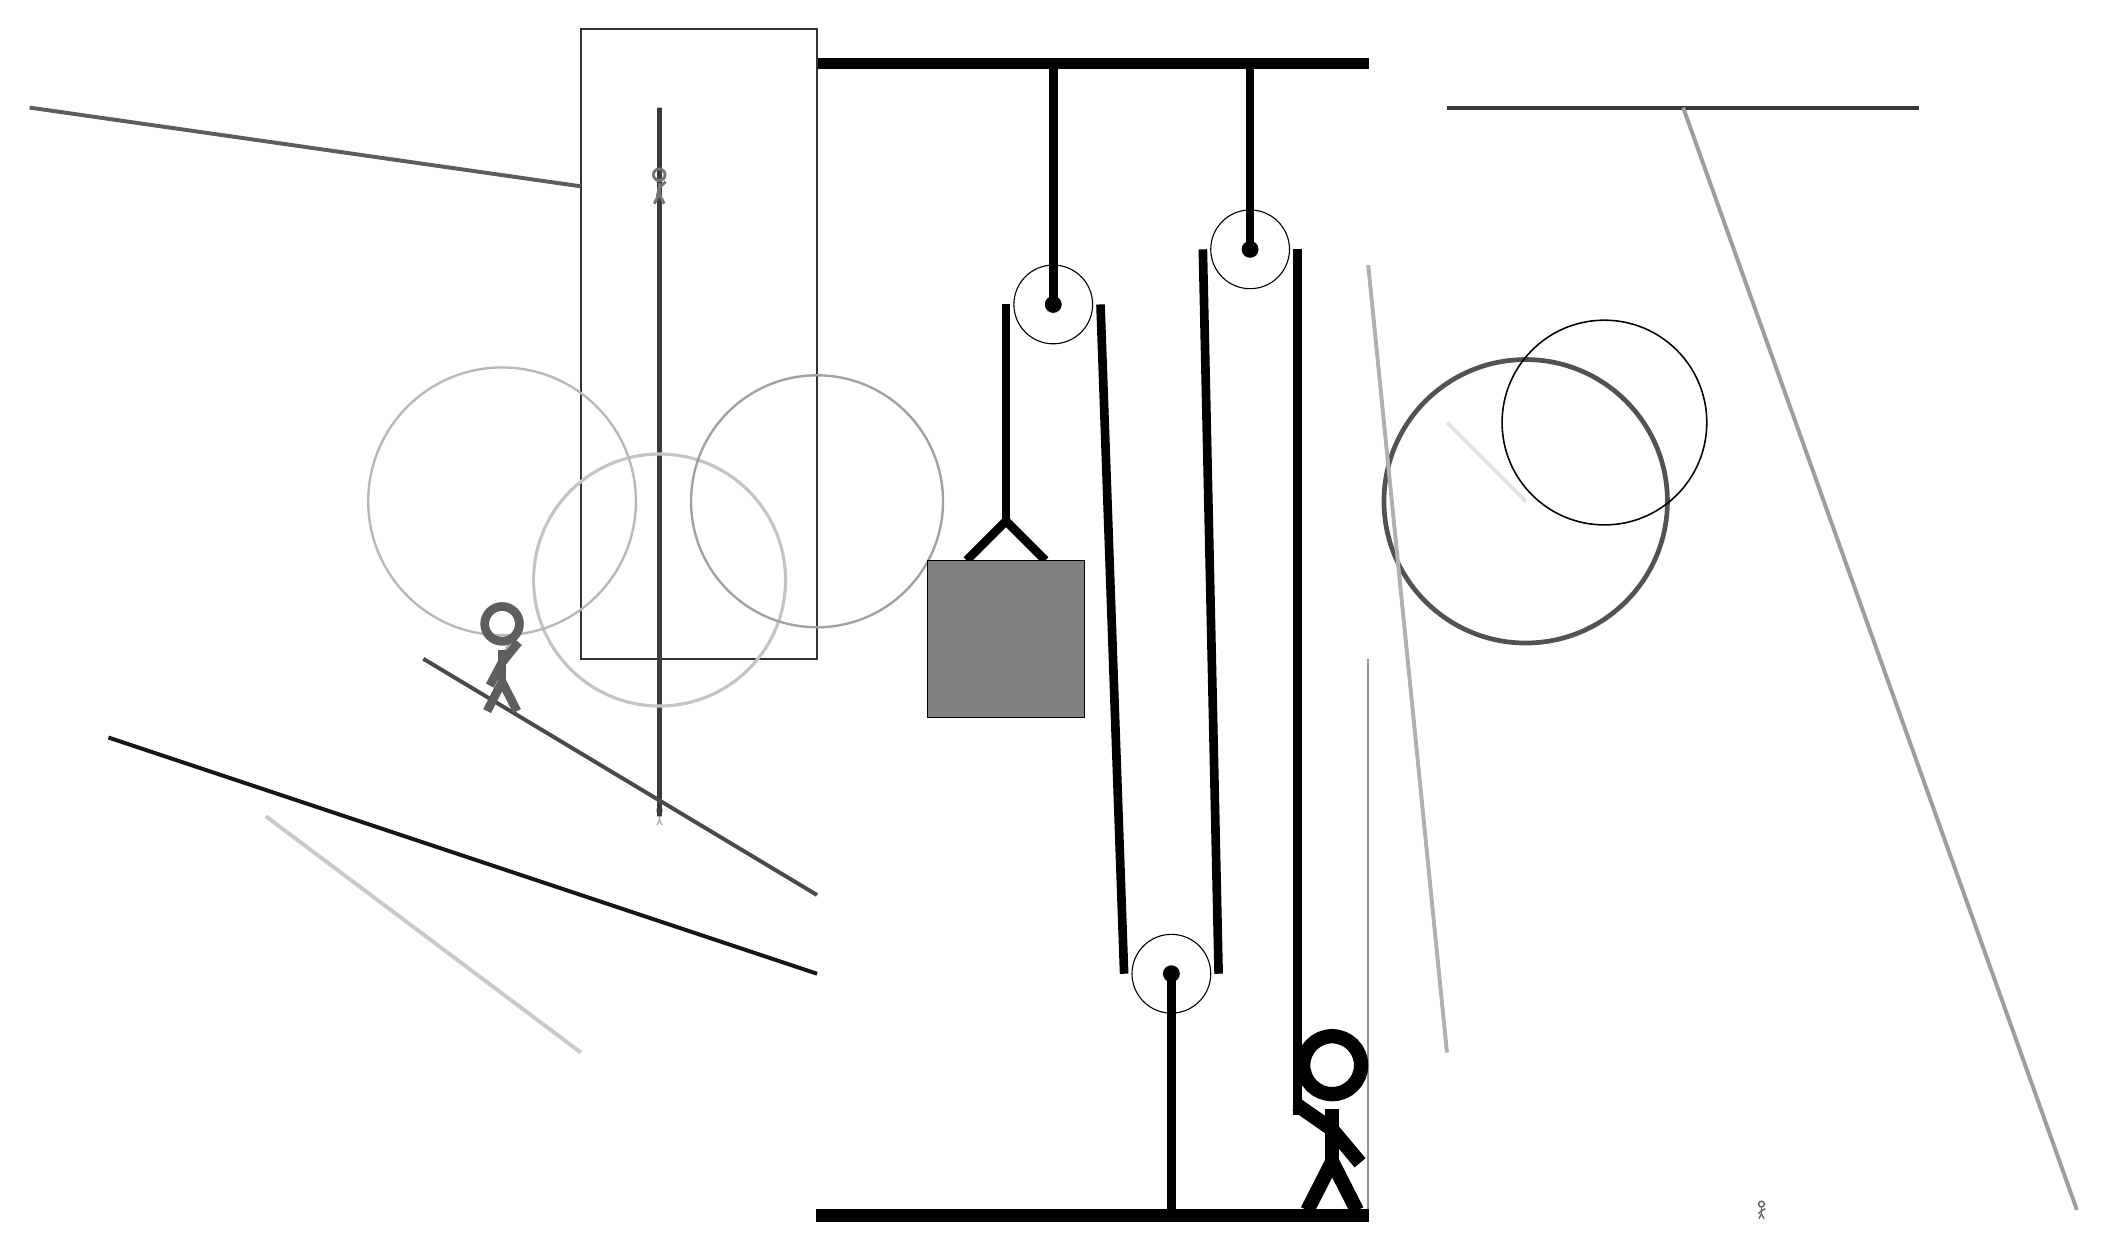
\begin{tikzpicture}
			%%%%% START %%%%%
			
			\draw[fill=black] (-2, 11.5) rectangle (5, 11.625);
			
			\draw (1, 8.5) circle (0.5);
			\draw[fill=black] (1, 8.5) circle (0.1);
			\draw[line width=1.1mm]  (1, 11.5) -- (1, 8.5);
			
			\draw[fill=white](2.5, 0.0) circle (0.5);
			\draw[fill=black] (2.5, 0.0) circle (0.1);
			\draw[line width=1.1mm]  (2.5, -3) -- (2.5, 0.0);
			
			\draw[fill=white](3.5, 9.2) circle (0.5);
			\draw[fill=black] (3.5, 9.2) circle (0.1);
			\draw[line width=1.1mm] (3.5, 11.5) -- (3.5, 9.2);
			
			\node[line width=0.7mm, color=black!32] at (-4, 2) {\Strichmaxerl[1][87][85]};
			
			\draw[line width=0.3mm, color=black!80] (-2, 4) rectangle (-5, 12);
			\draw[line width=0.7mm, color=black!77] (-4, 2) rectangle (-4, 11);
			\draw [line width=0.4mm, color=black!85](-7, 1) circle (0.0);
			\draw[line width=0.3mm, color=black!42] (5, 4) rectangle (5, -3);
			\draw[line width=0.5mm, color=black!21](-5, -1) -- (-9, 2);
			
			\draw [line width=0.4mm, color=black!23](-4, 5) circle (1.6);
			\draw [line width=0.3mm, color=black!37](-2, 6) circle (1.6);
			\draw [line width=0.3mm, color=black!28](-6, 6) circle (1.7);
			\draw [line width=0.6mm, color=black!68](7, 6) circle (1.8);
			\draw[line width=0.5mm, color=black!78](6, 11) -- (12, 11);
			
			\node[line width=0.6mm, color=black!32] at (-6, 4) {\Strichmaxerl[6][62][60]};
			\draw[line width=0.5mm, color=black!64](-5, 10) -- (-12, 11);
			
			\draw[line width=0.5mm, color=black!71](-2, 1) -- (-7, 4);
			\draw [line width=0.2mm, color=black!99](8, 7) circle (1.3);
			\node[line width=0.3mm, color=black!54] at (-4, 10) {\Strichmaxerl[2][77][42]};
			
			\node[line width=0.4mm, color=black!63] at (-6, 4) {\Strichmaxerl[6][62][51]};
			\draw[line width=0.5mm, color=black!38](9, 11) -- (14, -3);
			\draw[line width=0.5mm, color=black!91](-2, 0) -- (-11, 3);
			
			\draw[line width=0.5mm, color=black!31](6, -1) -- (5, 9);
			\draw[line width=0.5mm, color=black!11](7, 6) -- (6, 7);
			
			\node[line width=0.2mm, color=black!61] at (10, -3) {\Strichmaxerl[1][46][24]};
			
			\draw[line width=1.1mm] (-0.1, 5.25) -- (0.4, 5.75) -- (0.9, 5.25);
			\draw[fill=black!50] (-0.6, 5.25) rectangle (1.4, 3.25);
			
			\draw[line width=1.1mm] (0.4, 8.5) -- (0.4, 5.75);
			\centerarc[line width=1.1mm](1, 8.5)(0:180:0.6);
			\draw[line width=1.1mm](1.6, 8.5) -- (1.9, 0.0);
			\centerarc[line width=1.1mm](2.5, 0.0)(180:360:0.6);
			\draw[line width=1.1mm](3.1, 0.0) -- (2.9, 9.2);
			\centerarc[line width=1.1mm](3.5, 9.2)(0:180:0.6);
			\draw[line width=1.1mm](4.1, 9.2) -- (4.1, -1.8);
			
			\node at (4.5, -1.9) {\Strichmaxerl[10][-35][-50]};
			
			\draw[fill=black] (-2, -3) rectangle (5, -3.15);
			
			%%%%% END %%%%%
		\end{tikzpicture}
	\end{figure}	
\end{document}